\documentclass[12pt,a4paper]{article}
\usepackage[utf8]{inputenc}
\usepackage{amsmath}
\usepackage{amsfonts}
\usepackage{amssymb}
\usepackage{graphicx}
\usepackage{tabularx}
\usepackage{booktabs}
\usepackage{xcolor}
\usepackage{array}
\usepackage{colortbl}
\usepackage{float}
\usepackage{geometry}
\usepackage{tikz}
\usetikzlibrary{shapes.geometric, arrows}

\title{Divisive Synthesis\\
\small{1st Edition}}
\author{Digital Down}

\begin{document}

\maketitle

\begin{abstract}
This paper introduces and explores Divisive Synthesis, an approach in sound synthesis that utilizes the last unexplored common arithmetic operation in audio synthesis. While additive, subtractive and multiplicative synthesis have long been staples in the field, divisive synthesis has remained conspicuously absent.

\end{abstract}

\section{Introduction}
 Despite the field's long history of innovation, Divisive Synthesis emerges as an unexplored "low-hanging fruit," offering a rich palette of timbral possibilities with relatively simple implementation. This research introduces a new synthesis technique but also serves as a reminder that even in mature fields, there remains simple concepts that have not been fully realized.

\subsection{Historical Context}

\subsubsection{Additive Synthesis}
Additive Synthesis, one of the oldest methods of sound synthesis, is rooted in Fourier's theorem, which states that any periodic waveform can be constructed from a sum of sinusoidal waves of various frequencies, amplitudes, and phases \cite{Additive}.

The fundamental principle of Additive Synthesis can be expressed mathematically as:

\begin{equation*}
y(t) = \sum_{n=1}^{N} A_n \sin(2\pi f_n t + \phi_n)
\end{equation*}

where $y(t)$ is the resulting waveform, $A_n$ is the amplitude of the $n$th partial, $f_n$ is its frequency, and $\phi_n$ is its phase.

\subsubsection{Subtractive Synthesis}
Subtractive Synthesis, popularized in the 1960s and 1970s with the advent of analog synthesizers, operates on the principle of filtering harmonically rich waveforms \cite{Subtractive}.

The process can be described as:

\begin{equation*}
y(t) = H(f) * x(t)
\end{equation*}

where $y(t)$ is the output signal, $x(t)$ is the input signal, and $H(f)$ is the transfer function of the filter.

\subsubsection{Multiplicative Synthesis (Ring Modulation)}
Multiplicative Synthesis, often referred to as Ring Modulation, involves the multiplication of two input signals \cite{Multiplicative}. The basic form is expressed as:

\begin{equation*}
y(t) = x_1(t) * x_2(t)
\end{equation*}

where $y(t)$ is the output signal, and $x_1(t)$ and $x_2(t)$ are the input signals.

\subsubsection{Divisive Synthesis}

Divisive Synthesis represents a novel approach to sound generation, operating on the principle of dividing one waveform by another. The fundamental equation for Divisive Synthesis can be expressed as:

\begin{equation*}
y(t) = \frac{x_1(t)}{x_2(t)}
\end{equation*}

where $y(t)$ is the output signal, $x_1(t)$ is the numerator waveform, and $x_2(t)$ is the denominator waveform.
\section{Methodology}

\subsection{Waveform Generation}
Two distinct waveforms are generated for the Divisive Synthesis process:

\begin{enumerate}
    \item Active Waveform ($W_a$): This is the primary waveform that will be divided.
    \item Divisive Waveform ($W_d$): This waveform's samples will serve as the divisors in the synthesis process.
\end{enumerate}

\subsection{Divisive Power}

\begin{enumerate}
    \item The divisive waveform's samples are normalized to a range determined by a parameter called "divisive power" ($P_d$). This process can be expressed mathematically as:
    
    \begin{equation*}
    W_{d_{norm}}(t) = \frac{W_d(t)}{2^{15}} \cdot 2^{P_d - 1}
    \end{equation*}
    
    where $W_d(t)$ is the original 16-bit sample value at time $t$, and $P_d$ is the divisive power.
    
Table \ref{tab:divisive_power_ranges} illustrates the relationship between divisive power and the corresponding acceptable ranges for the divisive waveform.

\begin{table}[H]
\centering
\rowcolors{2}{gray!10}{white}
\begin{tabular}{|l|r@{\hspace{0.5em}}c@{\hspace{0.5em}}l|}
\hline
\rowcolor{white}
Divisive Power & \multicolumn{3}{c|}{Acceptable Range} \\
\hline
1 & -1 & to & 1 \\
2 & -2 & to & 2 \\
3 & -4 & to & 4 \\
4 & -8 & to & 8 \\
5 & -16 & to & 16 \\
6 & -32 & to & 32 \\
7 & -64 & to & 64 \\
8 & -128 & to & 128 \\
9 & -256 & to & 256 \\
10 & -512 & to & 512 \\
11 & -1024 & to & 1024 \\
12 & -2048 & to & 2048 \\
13 & -4096 & to & 4096 \\
14 & -8192 & to & 8192 \\
15 & -16384 & to & 16384 \\
16 & -32768 & to & 32768 \\
\hline
\end{tabular}
\caption{Acceptable Ranges for Each Divisive Power}
\label{tab:divisive_power_ranges}
\end{table}

As shown in Table \ref{tab:divisive_power_ranges}, the acceptable range for the divisive waveform's samples expand exponentially as the divisive power increases. This relationship can be expressed mathematically as:

\begin{equation*}
\text{Range} = [-2^{(P_d - 1)}, 2^{(P_d - 1)}]
\end{equation*}

where $P_d$ is the divisive power.

    \item Rounding: The values are then rounded to the nearest integer:
    
    \begin{equation*}
    W_{rounded}[n] = \text{round}(W_{result}[n])
    \end{equation*}
\end{enumerate}
\subsection{Division Operation}
The core of Divisive Synthesis lies in the sample-by-sample division of the input signals. This operation is performed for each sample in the digital domain:

\begin{equation*}
y[n] = \frac{x_1[n]}{x_2[n]}
\end{equation*}

where $n$ is the sample index.

\subsubsection{Zero Conditional}
One of the primary challenges in implementing Divisive Synthesis is handling division by zero. To address this, a conditional statement is used to skip division when the denominator is zero. This strategy can be expressed mathematically as:

\begin{equation*}
y(t) = \begin{cases} 
      \frac{x_1(t)}{x_2(t)} & x_2(t) \neq 0 \\
      x_1(t) & x_2(t) = 0
   \end{cases}
\end{equation*}

where $x_1(t)$ is the sample of the active waveform at time $t$, and $x_2(t)$ is the sample of the divisive waveform at time $t$.


\subsection{Post Processing}
After the division operation, the resulting waveform undergoes two final processing steps:

\begin{enumerate}
    \item Rounding: Each sample's division result is rounded to the nearest integer to maintain compatibility when converting the raw audio values into output:
    
    \begin{equation*}
    W_{rounded}[n] = \text{round}(_{result}[n])
    \end{equation*}


    \item Normalization: All samples are normalized to ensure it fits within the desired bit depth range (typically 16-bit). This can be expressed as:
    

    \begin{equation*}
    W_{final}[n] = \frac{W_{rounded}[n]}{\max(|W_{rounded}|)} \cdot (2^{15} - 1)
    \end{equation*}
\end{enumerate}

where $W[n]$ represents the nth sample in the sequence of samples.

\subsection{Output}
The division operation in the time domain leads to complex spectral interactions. Consider two sinusoidal inputs:

\begin{equation*}
x_1(t) = A_1 \sin(2\pi f_1 t)
\end{equation*}
\begin{equation*}
x_2(t) = A_2 \sin(2\pi f_2 t)
\end{equation*}

The resulting output can be expressed as:

\begin{equation*}
y(t) = \frac{A_1 \sin(2\pi f_1 t)}{A_2 \sin(2\pi f_2 t)}
\end{equation*}

This operation leads to a series expansion involving Chebyshev polynomials of the second kind, resulting in a rich harmonic spectrum \cite{Chebyshev}.

\section{Conclusion}

\begin{figure}[h]
\centering
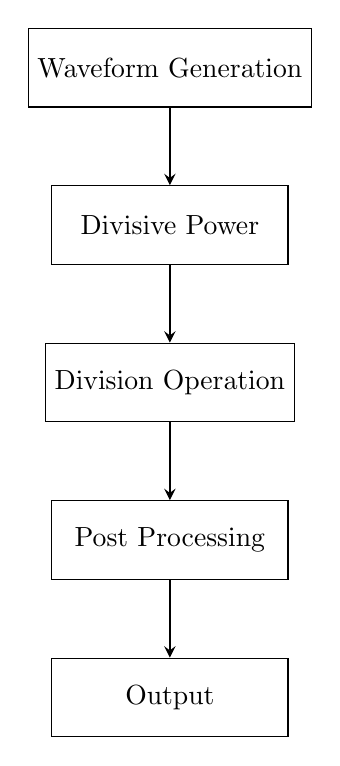
\begin{tikzpicture}[node distance=2cm]
\tikzstyle{process} = [rectangle, minimum width=3cm, minimum height=1cm, text centered, draw=black]
\tikzstyle{arrow} = [thick,->,>=stealth]

\node (start) [process] {Waveform Generation};
\node (power) [process, below of=start] {Divisive Power};
\node (division) [process, below of=power] {Division Operation};
\node (post) [process, below of=division] {Post Processing};
\node (output) [process, below of=post] {Output};

\draw [arrow] (start) -- (power);
\draw [arrow] (power) -- (division);
\draw [arrow] (division) -- (post);
\draw [arrow] (post) -- (output);
\end{tikzpicture}


\end{figure}

Divisive Synthesis stands as a testament to the ongoing potential for innovation in audio synthesis. It reminds us that even in mature fields, there remain fundamental concepts waiting to be explored, inviting further exploration and creative applications in sound design.

\printbibliography
\begin{thebibliography}{9}
\bibitem{Additive} Smith, Julius O. 
Spectral Audio Signal Processing,
W3K Publishing, http://books.w3k.org/,
ISBN 978-0-9745607-3-1.
\bibitem{Subtractive} Bates, Jon. "The History of the World: Part One, Subtractive Synthesis". Amiga Format, no. 4, 1989 Nov 01, 1989/11/01/, pp. 98.
\bibitem{Multiplicative} Bode, Harald. (1984). History of Electronic Sound Modification. Journal of the Audio Engineering Society. 32. 730-739. 
\bibitem{Chebyshev}Chebyshev, P. L. (1854). "Théorie des mécanismes connus sous le nom de parallélogrammes". Mémoires des Savants étrangers présentés à l'Académie de Saint-Pétersbourg (in French). 7: 539–586.
\end{thebibliography}
\end{document}